% !TeX spellcheck = en_GB

\section{From Individual Neurons to Spiking Neural Networks}
\label{sec:neuron_models}

The equations from the previous section model the basic electrophysiological properties of individual neurons.
Of course, a single neuron on its own does not give rise to animal behaviour.
Hence, in this section, we discuss how individual neurons can be used to form neural networks.
We provide an overview of synaptic transmission, the process underpinning neural information transfer, followed by a discussion of idealised neuron and synapse models that lessen the computational burden of simulating biological systems.
We close with a short discussion of spiking neural networks and population tuning---the latter shedding some light onto the role that individual neurons play in a network.


\subsection{Synaptic Transmission}
\label{sec:synaptic_transmission}

So far, our descriptions of neural dynamics assumed that neurons receive inputs through artificially injected currents $J(t)$.
%While this can be experimentally achieved using a microelectrode and a precision power supply,
Of course, this does not explain how neurons receive inputs \emph{in vivo}.
As we mentioned in our overview in \Cref{sec:neurons_overview}, the interface between two neurons is called a \emph{synapse}.
Neuroscientists distinguish two synapse types: electrical and chemical.


\subsubsection{Electrical synapses}
In adult vertebrates, electrical synapses are much less common than chemical synapses.
Still, they play an important role in some mammalian brain areas, including the retina and the inferior olive in the cerebellum \citep[Chapter~5]{meriney2019synaptic}.

Electrical synapses directly connect two neurons through specialised ion channels, so-called \emph{gap junctions}.
These channels typically allow a bidirectional exchange of ions between the intracellular fluids.
Correspondingly, neurons connected via gap junctions can be modelled using the same techniques as multi-compartment models (eq.~\ref{eqn:multi_comp_current}; \cite{kandel2012principles}, Chapter~8).

\subsubsection{Chemical synapses}
Neurons coupled via chemical synapses are electrically isolated.
The synapse establishes a unidirectional information flow and only passes on superthreshold signals.
The transmitting and receiving neurons are generally referred to as \enquote{pre-synaptic} and \enquote{post-synaptic neurons}, respectively.
To save some space, we use the terms pre- and post-neurons.
Similarly, the synapse is divided into the \enquote{pre-} and \enquote{post-synapse}.

\begin{figure}
	\includegraphics{media/chapters/02_modelling/02_02/synapse.pdf}%
	\caption[Synaptic transmission in a chemical synapse]{Synaptic transmission in a chemical synapse. Grey line in the membrane potential traces is the spike onset. See text for a description. Inspired by \citet[Figure~8-8B-C, p.~185]{kandel2012principles}.}
	\label{fig:synapse}
\end{figure}

As illustrated in \Cref{fig:synapse}, action potentials arriving at axon terminal, trigger the release of \emph{neurotransmitter} molecules.
These traverse the nanometer-scale gap between the pre- and post-synapse, the \emph{synaptic cleft}, and temporarily bind to post-synaptic receptors specific to that neurotransmitter type.
This---directly or indirectly---causes ion channels in the post-neuron to open.
In turn, the permeability of the post-neuron for that particular ion species changes.

The resulting synaptically mediated membrane potential fluctuations are called \emph{post-synaptic potentials} (PSPs).
Depending on the type of ion channels opened or closed, the PSP can either drive the neuron towards more positive voltages (if sodium channels are opened), or negative voltages (e.g., if potassium or chloride channels are opend).
Positive PSPs are referred to as \emph{excitatory} (EPSP), negative changes as \emph{inhibitory} (IPSP).
%Correspondingly, we distinguish excitatory and inhibitory post-synaptic potentials (EPSPs) and (IPSPs).

Whether a pre-neuron acts excitatorily or inhibitorily on a post-neuron depends on the kind of neurotransmitter released by the pre-neuron, as well as the specific receptors and ion channels in post-neuron.
%Typically, each neurotransmitter either has an inhibitory or excitatory effect.
For example, the Gamma-Aminobutyric acid (GABA) neurotransmitter is primarily inhibitory (via GABA\textsubscript{A} or GABA\textsubscript{B} receptors), whereas Glutamic acid (Glutamate) is mostly excitatory (via AMPA or NMDA receptors; \cite{kandel2012principles}, Chapter~10).

Importantly, the mixture of neurotransmitters is the same across all axonal branches of a neuron.
This is known as \emph{Dale's principle}\index{Dale's principle} \citep{strata1999dale,eccles1986chapter}.
Put simply, individual neurons typically either act excitatorily or inhibitorily on their post-neurons.%
\footnote{This characterisation of Dale's principle is useful, but technically incorrect. For example, a pre-synapse releasing glutamate typically excites post-neurons, but inhibits special neurons with inhibitory glutamate receptors \citep{cleland1996inhibitory}.
Additionally, synapses could release both excitatory and inhibitory neurotransmitters.
%Furthermore, Dale's principle solely states that the \emph{mixture} of neurotransmitters is uniform within the axonal branches of a neuron \citep{strata1999dale,eccles1986chapter}. In theory, the pre-synapse could release both excitatory and inhibitory neurotransmitters.
}
We hence refer to neurons---and not just individual synapses---as being excitatory or inhibitory.

\begin{figure}
	\centering
	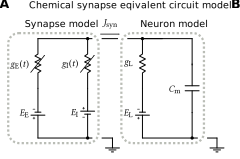
\includegraphics[scale=0.3333]{media/chapters/02_modelling/02_02/synapse_model.pdf}%
	\includegraphics{media/chapters/02_modelling/02_02/synapse_model_traces.pdf}%
	{\phantomsubcaption\label{fig:synapse_model_circuit}}%
	{\phantomsubcaption\label{fig:synapse_model_traces}}%
	\caption[The conductance-based synapse model]{The conductance-based synapse model.
	\textbf{(A)} Circuit diagram of a passive cell membrane with synaptically controlled excitatory and inhibitory conductance-based channels.
	\textbf{(B)} Illustrative voltage, current, and conductance traces. \emph{Top:} Excitatory and inhibitory channel conductances after a pre-synaptic action potential (grey dashed line). \emph{Middle:} Resulting excitatory and inhibitory post-synaptic potentials. \emph{Bottom:} Corresponding excitatory and inhibitory post-synaptic currents.}
	\label{fig:synapse_model}
\end{figure}

\subsubsection{Conductance-based chemical synapse model}
Most gated ion channels can be modelled as a voltage-resistor pair with variable conductance per receptor type \citep{roth2009modeling}.
This is depicted in \Cref{fig:synapse_model} for generic \enquote{excitatory} and \enquote{inhibitory} receptors.
Mathematically, the post-synaptic current $J_\mathrm{syn}(t)$ flowing from the synapse into the neuron is given as
\begin{align}
	J_\mathrm{syn}(t) &=
		  g_\mathrm{E}(t) \bigl(E_\mathrm{E} - v(t)\bigr)
		+ g_\mathrm{I}(t) \bigl(E_\mathrm{I} - v(t)\bigr) \,.
	\label{eqn:conductance_synapse}
\end{align}
Here, $E_\mathrm{E}$ and $E_\mathrm{I}$ are the equilibrium potentials of the gated ion channels.
These potentials are not necessarily equal to ion reversal potentials (\Cref{tbl:nernst}).
For example, NMDA and AMPA channels conduct both $\mathrm{Na^+}$ and $\mathrm{K^+}$, resulting in $E_\mathrm{E} \approx \SI{0}{\milli\volt}$ \citep[Chapter~10]{kandel2012principles}.
%All receptors with the same reversal potential are summarised as single channel in the equivalent circuit.
%Correspondingly, $g_\mathrm{E}$ and $g_\mathrm{I}$ are the sum over the state of multiple post-neurons (similar to \Cref{fig:electrical_circuit_individual_channels}).

\subsubsection{Synaptic dynamics and weights}
The time course of the conductance $g(t)$ depends on the neurotransmitter and receptor type.
Generally speaking, as illustrated in \Cref{fig:synapse_model_traces}, the conductance rises quickly after a spike is received, and decays slowly as the neurotransmitter unbinds from the receptors.
Receptors directly controlled by neurotransmitters acting as ligands (\Cref{fig:synapse}) tend to have relatively short time-constants between $1$ and \SI{100}{\milli\second} \citep{jones2014neurotransmitter}.
Some receptors (e.g., \enquote{metabotropic receptors}) rely on indirect chemical cascades, leading to longer time-constants \citep[Chapter~14]{meriney2019synaptic}; this is not captured well by the models we present here \citep{roth2009modeling}.

\begin{figure}
	\includegraphics{media/chapters/02_modelling/02_02/synapse_filter_examples.pdf}
	{\phantomsubcaption\label{fig:synapse_filter_examples_time_constants}}%
	{\phantomsubcaption\label{fig:synapse_filter_examples_traces}}%
	\caption[Second- and first-order exponential synaptic low-pass filter dynamics]{Illustration of the second- and first-order exponential synaptic low-pass filter dynamics. \textbf{(A)} Impulse response of the second-order dynamics for different $\tau_1$ and $\tau_2$. \emph{Top:} visualisation of the time-constants used below. Swapping $\tau_1$ and $\tau_2$ does not change the dynamics (grey crosses). \emph{Bottom:} Impulse response of the filters (responses normalised to equal area), circles are the peaks. \textbf{(B)} Illustration of post-synaptic conductance traces (\emph{bottom}) according to \Cref{eqn:low_pass_second_order,eqn:low_pass_first_order} for two pre-neurons producing action-potentials (\emph{top}) connected with two different synaptic weights $w_1$, $w_2$.}
\end{figure}

Ligand-gated receptor dynamics are often modelled as a second-order linear dynamical system.
Let $t_{ij}$ denote the time of the $j$th pre-synaptic spike arriving from the $i$th pre-neuron, and let $\tau_1$, $\tau_2$ denote the rise and delay times (\Cref{fig:synapse_filter_examples_time_constants}).
We have \citep{roth2009modeling}:
\begin{align}
	\dot g_1(t) &= -\frac{g_1(t)}{\tau_\mathrm{1}} + g_2(t) \,, &
	\dot g_2(t) &= -\frac{g_2(t)}{\tau_\mathrm{2}} + \sum\nolimits_{i} \alpha w_i \sum\nolimits_{j} \delta(t_{ij} - t) \,,
	\label{eqn:low_pass_second_order}
\end{align}
where $\delta(t)$ is the Dirac-delta, and $\alpha$ is a scaling factor such that the scalar $w_i$ corresponds to the peak value of $g_1(t)$ for a single action potential received from pre-neuron $i$ (\Cref{fig:synapse_filter_examples_traces}).
For $\tau_1 = \tau_2$ this type of synaptic dynamics follow the so-called \emph{alpha function}.

Notably, the scalar $w_i$ is referred to as \emph{synaptic weight} in computational modelling, or as \emph{synaptic strength} in neuroscience.
This scalar summarises various biological processes that determine the average response of the post-neuron to an action-potential received from the $i$th pre-neuron.
For example, synaptic strength can depend on the amount of neurotransmitter released in the pre-synapse, or the ion-channel density in the post-synapse \citep[Chapter~12]{kandel2012principles}.
In this context, the term \emph{synaptic plasticity} refers to a change in synaptic strength over time.
This plays a key role in learning---we discuss this in more detail in Chapter~5.


Typically, the rise-time of $g(t)$ is relatively short.
Correspondingly, the second-order low-pass filter can be approximated by a first-order dynamical system with decay-time $\tau$.
Mathematically, and as depicted the lower portion of \Cref{fig:synapse_filter_examples_traces}, the dynamics are
\begin{align}
	\dot g(t) &= -\frac{g(t)}{\tau} + \sum\nolimits_{i}  w_i \sum\nolimits_{j} \delta(t_{ij} - t) \,.
	\label{eqn:low_pass_first_order}
\end{align}

\subsubsection{Synaptic dynamics as filters}
The above synaptic dynamics (eqs.~\ref{eqn:low_pass_second_order}, \ref{eqn:low_pass_first_order}) are linear time-invariant (LTI) systems.
%of the form $\dot{\vec g}(t) = \mat A{\vec g(t)} + \mat B u(t)$, where $\mat A \in \mathbb{R}^{n \times n}$ is a state-transition matrix, $\mat B \in \mathbb{R}^{n \times 1}$ is the input matrix, and $u(t)$ is the input in the form of weighted pre-synaptic spike events; the output of the system (i.e., the conductance) is simply the first state-dimension $g_1$.
LTI systems are fully characterised by their \emph{impulse response} $h(t)$ and can be replaced by a convolution (\enquote{$\ast$}) between $h(t)$ and the weighted input spike-train $u(t)$:
\begin{align}
	g(t)
		&= (h \ast u)(t)
		 = \int_0^t h(\tau) u(\tau - t) \,\mathrm{d}\tau
		 = \int_0^t h(\tau) \sum\nolimits_{i}  w_i \sum\nolimits_{j} \delta(t_{ij} - \tau) \,\mathrm{d}\tau \,.
	\label{eqn:synapse_impulse}
\end{align}
For the first-order dynamics in \cref{eqn:low_pass_first_order}, the impulse response is $h(t) = \exp(-t/\tau)$ for $t \geq 0$ (and $h(t)= 0$ if $t < 0$); impulse responses of the second-order system are depicted in \Cref{fig:synapse_filter_examples_time_constants}.
Convolutions such as \cref{eqn:synapse_impulse} can alternatively be expressed as multiplication of the frequency contents of the impulse response $h(t)$ and the input spike-train $u(t)$:
\begin{align}
	g(t) &= \mathcal{F}^{-1} \bigl(\mathcal{F}(h) \mathcal{F}(u) \bigr)(t) \,,
\end{align}
where $\mathcal{F}$ is the forward Fourier transformation, and $\mathcal{F}^{-1}$ its inverse.
From this signal-processing perspective, the synaptic dynamics attenuate frequencies in the input spike-train; they act as a \emph{filter}.
The synaptic dynamics discussed so far attenuate low frequencies far less than higher frequencies; they are thus referred to as \emph{low-pass filters}.

% TODO: Talk about filters in general
% TODO: Provide some example synaptic time constants

\newpage

\subsection{Simplified Neuron Models}
\label{sec:simplified_neuron_models}

The models discussed in the previous section describe indiviudal neurons at a relatively low level of abstraction.
This incurs a high computational cost, especially when considering detailed compartemental neurons with Hodgkin-Huxley-like super-threshold dynamics.

Fortunately, important electrophysiological properties of neurons can be captured by less detailed, computationally inexpensive, models \citep[cf.][Chapter~14]{koch1999biophysics}.
For example, the Izhikevich \citep{izhikevich2004which} and Adaptive Exponential \citep{brette2005adaptive} point neuron models require only two state variables, but are capable of reproducing spike patterns observed in nature.
Here, we focus on the even simpler \enquote{leaky integrate-and-fire} (LIF) model\index{leaky integrate-and-fire model}.

\subsubsection{The leaky integrate-and-fire model}

\begin{figure}[t]
	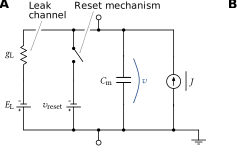
\includegraphics[scale=0.3333]{media/chapters/02_modelling/02_02/lif_circuit.pdf}%
	\kern-0.25cm\includegraphics{media/chapters/02_modelling/02_02/lif_traces.pdf}
	\caption[Equivalent circuit diagram and membrane potential trace of a LIF neuron]{Equivalent circuit diagram and membrane potential trace of a LIF neuron. \textbf{(A)} The LIF model consists of a capacitative membrane with a \enquote{leak} channel. A reset mechanism clamps \vMem to the reset potential \vReset. \textbf{(B)} Membrane potential trace (\emph{top}) for rectangle pulse current inputs (\emph{middle}).  Vertical dashed lines are spike events. The bottom graph depicts the remaining refractory period.}
	\label{fig:lif}
\end{figure}

%\footnote{Extensions to the LIF model include the quadratic and exponential integrate-and-fire models (QIF and EIF, respectively). Hence, LIF is sometimes read as \enquote{linear integrate-and-fire}. Furthermore, there is the IF model, that does not include a leak channel, sometimes also called nLIF (non-leaking).}
A variant of the LIF model---lacking refractoriness---dates back to \citet{lapicque1907recherches}.
Just like the Hodgkin-Huxley model (\Cref{sec:neural_dynamics}), the LIF neuron is based on a capacitive membrane with a leak channel.
The input current is integrated by the capacitor, which, at the same time, is discharged through the leak channel:
\begin{align}
	\CMem \dot{\vMem}(t) =
		\gL \bigl(\EL - \vMem(t)\bigr) + J(t) \,,
	\label{eqn:lif}
\end{align}
where \gL is the leak conductance, \EL is the leak reversal potential, and $J(t)$ is a (synaptic) current injected into the membrane.
Unlike the Hodgkin-Huxley model, the dynamics of the system do not model spike production; \enquote{firing} is handled outside the dynamical system. 
Once $\vMem(t)$ reaches a threshold $\vTh$, a spike event is recorded and \vMem is held at the \emph{reset potential} \vReset for the duration of the refractory period \tauRef.
This is depicted in \Cref{fig:lif}.

\subsubsection{Response curve}

\begin{figure}
	\centering
	\includegraphics{media/chapters/02_modelling/02_02/neuron_voltage_traces.pdf}
	\caption[Voltage traces for the LIF and Hodgkin-Huxley neuron model]{Voltage traces (\emph{top}) for the LIF and a Hodgkin-Huxley-type neuron dynamics described by \citet{traub1991neuronal} given a current ramp input~(\emph{bottom}). Dashed vertical lines correspond to spike events. Dotted line is the resting potential at $\EL=\SI{-65}{\milli\volt}$. Both neurons have a membrane capacitance of $C_\mathrm{m} = \SI{200}{\pico\farad}$ and a leak conductance of $g_\mathrm{L} = \SI{10}{\nano\siemens}$. \textbf{(A)} The LIF neuron model does not account for spike production; the voltage is simply reset to $v_\mathrm{reset} = \SI{-85}{\milli\volt}$ for $\tauRef = \SI{2}{\milli\second}$ once the membrane potential passes the threshold at $v_\mathrm{th} = -\SI{55}{\milli\volt}$. \textbf{(B)} Same experiment for a Hodgkin-Huxley neuron. Notably, the super-threshold dynamics of the Hodgkin-Huxley model action potentials and the first spike appears significantly earlier compared to the LIF neuron.}
	\label{fig:neuron_voltage_traces}
\end{figure}

\begin{figure}
	\centering
	\includegraphics{media/chapters/02_modelling/02_02/neuron_response_curves.pdf}%
	{\phantomsubcaption\label{fig:neuron_response_curves_lif}}%
	{\phantomsubcaption\label{fig:neuron_response_curves_hh}}%
	\caption[Response curves for the LIF and Hodgkin-Huxley-type neuron model]{Response curves (also called IF-curves) $G[J]$ for the LIF and Hodgkin-Huxley-type neuron model from \Cref{fig:neuron_voltage_traces}. Data extracted from the inter-spike-intervals of a current ramp experiment (sweep from \SIrange{0}{2}{\nano\ampere} over ten seconds at a \SI{10}{\micro\second} resolution). Although the LIF and Hodgkin-Huxley models have drastically different dynamics, their response curves are qualitatively similar.}
	\label{fig:neuron_response_curves}
\end{figure}

\begin{figure}
	\centering
	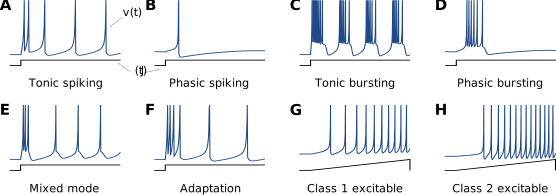
\includegraphics{media/chapters/02_modelling/02_02/izhikevich_whichmod_figure1.pdf}%
	{\phantomsubcaption\label{fig:izhikevich_whichmod_figure1a}}%
	{\phantomsubcaption\label{fig:izhikevich_whichmod_figure1b}}%
	{\phantomsubcaption\label{fig:izhikevich_whichmod_figure1c}}%
	{\phantomsubcaption\label{fig:izhikevich_whichmod_figure1d}}%
	{\phantomsubcaption\label{fig:izhikevich_whichmod_figure1e}}%
	{\phantomsubcaption\label{fig:izhikevich_whichmod_figure1f}}%
	{\phantomsubcaption\label{fig:izhikevich_whichmod_figure1g}}%
	{\phantomsubcaption\label{fig:izhikevich_whichmod_figure1h}}%
	\caption[Diversity of neural dynamics for constant or ramp input currents]{Diversity of neural dynamics for constant or ramp input currents. Each plot depicts membrane-potential traces $v(t)$ (\emph{top}) of the Izhikevich neuron model (with different parameters) for an input current $J(t)$ (\emph{bottom}). LIF neurons are only capable of behaviours \emph{A} and \emph{G}. Partially reproduced (dynamics for input pulses were skipped) with minor modifications from \citet{izhikevich2004which}. Electronic version of the figure and reproduction permissions freely available at \url{http://www.izhikevich.org}.}
	\label{fig:izhikevich_whichmod_figure1}
\end{figure}

\Cref{fig:neuron_voltage_traces} depicts a comparison between the Hodgkin-Huxley-type and LIF dynamics.
The reset and threshold potential of the LIF neuron model have been tuned to match the sub-threshold membrane potentials observed in the Hodgkin-Huxley neuron.
In both cases---apart from the obviously missing super-threshold dynamics---the inter-spike-interval decreases the larger $J$, leading to a higher spike rate.
This suggests a characterisation of neurons in terms of their \emph{response curve}\index{neuron!response curve} $G[J]$ (\Cref{fig:neuron_response_curves})
\begin{align}
	G[J] &= \lim_{T \to \infty} \frac{n_\mathrm{spikes}(J, T)}{T} \,, & \text{where } n_\mathrm{spikes}(J, T) &= \text{\#spikes for input $J$ over a period $T$} \,.
	\label{eqn:response_curve}
\end{align}
Of course, this only makes sense if we assume that the neuron has a non-zero steady-state activity for a constant superthreshold input current.
This is not necessarily true; neurons can exhibit complex behaviours that violate this assumption \citep{izhikevich2004which}.
For example, \emph{phasic} neurons only produce a limited number of spikes in response to an input step (Figure~\ref{fig:izhikevich_whichmod_figure1}B, D, E), while other neurons adapt to constant input currents over time, resulting in a reduction in frequency (Figure~\ref{fig:izhikevich_whichmod_figure1}F).
Still, neurons often behave \emph{tonically} (Figure~\ref{fig:izhikevich_whichmod_figure1}A, C, G, H), and can be reasonably well characterised in terms of a response curve.

Response curves and time-less \enquote{rate neurons} form the basis for artificial neural networks commonly used in machine learning. We discuss this in more detail later in this thesis.
Furthermore, we revisit temporal properties of the response curve when we discuss temporal tuning curves. % LEAVE SPACE HERE
% TODO add section references

\subsubsection{LIF response curve}
For most neuron models, it is impossible to derive a closed-form expression for the average spike rate $G[J]$ given a constant current $J$; there typically is no closed-form solution for $G[J]$. 
%\footnote{Very few differential equations posses closed-form solutions. Even slightly more complex models (e.g.,~first-order current-based synapses instead of constant $J$) require the analytic Lambert $\mathcal{W}$ function in the solution.}
Instead, we have to rely on the method suggested by \cref{eqn:response_curve}.
That is, we simulate the neural dynamics for a sufficiently long time-period and count the number of spikes $n_\mathrm{spikes}$.

The LIF neuron is a notable exception to this, as its subthreshold dynamics form a simple first-order linear dynamical system.
Using basic techniques for solving differential equations, the membrane potential \vMem at time $t$ for a constant input current $J$ is given as
\begin{align}
	v(t) &= \left(1 - e^{-\frac{t}{\tauMem}} \right) \left( \EL + \frac{J}{\gL} \right) + e^{-\frac{t}{\tauMem}} v(0) \,, &&\Rightarrow & \lim_{t \to \infty} v(t) &= \EL + \frac{J}{\gL} \,.
\end{align}
To compute the average spike rate, we need to know how long it takes to reach the threshold potential after a spike has been issued.
To this end, we simply solve $v(t_\mathrm{spike}) = \vTh$ with $v(0) = \vReset$ for $t_\mathrm{spike}$.
Keeping in mind that the neuron is held at the reset potential for $\tauRef$ seconds after every spike, and defining the threshold current $J_\mathrm{th} = (\vTh - \EL) \gL$, we have
\begin{align}
	\begin{aligned}
	G[J] &= \begin{cases}
		0 & \text{if } J \leq J_\mathrm{th} \,, \\
		\frac{1}{\tauRef + t_\mathrm{spike}} & \text{if } J > J_\mathrm{th} \,,
	\end{cases} & \quad
	\text{where }
%	J_\mathrm{th} &=
%		(\vTh - \EL) \gL \,, \\
	t_\mathrm{spike} &=
		-\tauMem \log\left(1 - \frac{(\vTh - \vReset) \gL}{(\EL - \vReset) \gL + J} \right) \,.
	\end{aligned}
	\label{eqn:lif_response_curve}
\end{align}
As depicted in \Cref{fig:neuron_response_curves_lif}, the predicted rate perfectly matches the empirical measurement.
Notably, the LIF response curve is qualitatively similar to that of the Hodgkin-Huxley neuron (\Cref{fig:neuron_response_curves_hh})---surprisingly so, as the dynamical systems differ wildly between the two models.
This makes LIF neurons a reasonable choice for simulating large-scale neurobiological systems at small computational costs (\cite{meunier2002playing}).

\subsubsection{Simplified LIF neuron}
A qualitatively equivalent form of the LIF neuron is given by normalising the voltages such that $\EL = 0$ and $\vTh = 1$, and furthermore setting $J_\mathrm{th} = 1$:
\begin{align}
	\dot v(t) &= -\frac{1}{\tauMem} v(t) + J(t) \,, &
	G[J] &= \begin{cases}
		0 & \text{if } J \leq 1 \,, \\
		\frac{1}{\tauRef - \tauMem \log\left(1 - \frac{1 - \vReset}{J-\vReset}\right)} & \text{if } J > 1 \,.
	\end{cases}
	\label{eqn:lif_simplified}
\end{align}
The primary advantage of this form is the reduction in mathematical operations compared to \cref{eqn:lif}.
This simplification (among other optimisations) is thu exploited by the neural network simulator \enquote{Nengo} to support large-scale spiking neural network simulations \citep{bekolay2014nengo}.
The downside is a reduced interpretability of the now unit-less $v(t)$ and $J(t)$.

\subsubsection{Current-based synapse models}
Another possible simplification---both in terms of computation and mathematical analysis---concerns the synapse model.
In conductance-based synapses (\Cref{sec:synaptic_transmission}) the current $J_\mathrm{syn}(t)$ explicitly depends on the membrane potential $\vMem(t)$.
Going back to \Cref{fig:synapse_model_traces}, one may notice that the post-synaptic currents can be approximated as a scaled version of the conductance \citep[cf.][]{roth2009modeling}.

This suggests modelling the post-synaptic current $J_\mathrm{syn}$ as a linear superposition of filtered spike events.
Let the synaptic weight $w_i$ denote the peak post-synaptic current.
Then, the first-order \emph{current-based} synapse model is given as (analogously for higher-order filters)
\begin{align}
	\dot J_\mathrm{syn}(t) &= -\frac{J_\mathrm{syn}(t)}{\tau} + \sum\nolimits_{i}  w_i \sum\nolimits_{j} \delta(t_{ij} - t) \,.
	\label{eqn:low_pass_first_order_current}
\end{align}
We compare conductance- and current-based synapse models in more detail in the next chapter.

\pagebreak

\subsection{Spiking Neural Networks}
\label{sec:neural_codes}

\begin{figure}
	\centering
	
\includegraphics{media/chapters/02_modelling/02_02/neural_networks.pdf}%
	{\phantomsubcaption\label{fig:neural_networks_a}}%
	{\phantomsubcaption\label{fig:neural_networks_b}}%
	{\phantomsubcaption\label{fig:neural_networks_c}}%
	\caption[Illustration of different neural network types]{Illustration of different neural network types. Blue circles depict individual neurons. \textbf{(A)} Feed-forward neural networks can be represented as acyclic graphs. \textbf{(B)} If the network connectivity contains cycles (e.g., the 5-2-4-5 cycle), the network is called \emph{recurrent}. Cycles can also be self-recurrences (e.g., neuron 6). \textbf{(C)} Artifical neurons (\emph{left}) process time-discrete samples. Spiking neurons (\emph{right}) are time-continous; they receive a weighted input spike train, filter it, and produce an output spike train.}
\end{figure}

% How to build neural networks
% Define feed-forward and recurrent neural networks
% But how to select the weights?
% Solution that artificial neural networks do
% But is this what biology does?
% Rate vs temporal coding debate -> Aaron

We are now well-equipped to construct and simulate spiking neural networks (SNNs).
In theory, we just take $n$ spiking neurons and connect them up according to synaptic weights $w_{ij}$. As mentioned before, these weights determine the connection strength between a pre-neuron $j$ and post-neuron $i$. Inputs are additive over multiple pre-neurons (eqs.~\ref{eqn:low_pass_first_order}, \ref{eqn:low_pass_first_order_current}).%
\footnote{This notion of synaptic weights $w_{ij}$ assumes that each neuron possesses a single synaptic input channel.
Hence, there is only a single synaptic weight matrix.
For neurons with multiple synaptic input channels we can simply use an individual weight matrix for each input channel. We discuss this in the next chapter.}

Mathematically, the \emph{weight matrix} $\mat W \in \mathbb{R}^{n \times n}$ is the adjacency matrix of a directed connectivity graph.%
\footnote{For convenience and computational efficiency, neurons are typically grouped into \enquote{layers}, \enquote{populations}, or \enquote{ensembles} (all terms are used synonymously).
Not all layers have connections among each other. Hence, $\mat W$ typically is a block-matrix that can be split into multiple sub-matrices.}
Networks with acyclic connectivity are called \emph{feed-forward} (\Cref{fig:neural_networks_a}); networks with cyclic connectivity are \emph{recurrent} (\Cref{fig:neural_networks_b}).
Feed-forward SNNs have finite memory.
Assuming plausible synaptic filters, their impulse response decays exponentially.
In contrast, and as we discuss later, recurrent networks can posses more interesting dynamics.

To actually simulate an SNN, we feed an external input (e.g., a set of currents or spike-trains) into the network and numerically integrate the coupled differential equations.
There are numerous general-purpose simulator software packages that do this efficiently, e.g., NEST \citep{gewaltig2007nest}, Brian \citep{stimberg2019brian}, GeNN \citep{yavuz2016genn}, or Nengo \citep{bekolay2014nengo}.

The most important question---and one that we pursue for the remainder of this thesis---is how to ultimately select $\mat W$.
For the artificial neural networks (ANNs) used in machine learning (\Cref{fig:neural_networks_c}), the astoundingly successful answer is to use stochastic gradient descent on a loss function $E$, i.e., $\dot{\mat W} = -\eta \nabla_{\mat W} E(\vec a_k, \vec {\hat a_k})$, where $\eta$ is a learning rate, $\vec a_k$ is the desired output activity for an input sample $\vec x_k$, and $\vec{\hat a_k}$ is the actual output \citep{lecun2015deep}.
For example, one common choice for the loss function is $E(\vec a_k, \vec {\hat a_k}) = \|\vec a_k - \vec{\hat a}_k\|^2$.

Similar gradient-descent global optimisation methods can be applied in the context of SNNs as well.
\Citet{hunsberger2018spiking} characterises the LIF response curve $G[J]$ in a network context and then trains an ANN that uses $G[J]$ as a nonlinearity.
The resulting $\mat W$ can then be used in a spiking context.
\Citet{goltz2020fast} optimise synaptic weights such that desired spike-timings are generated by a black-box spiking neural network simulator.

%Computational neuroscientists often distinguish between rate and temporal spike-codes, though the definitions of these concepts are quite vague.
%For example, \citet[Chapter~1]{gerstner2002spiking} list three different definitions of the term \enquote{rate code}, while \citet{abbott2001theoretical} list four definitions.
%Rates are estimated by either binning and counting, causal and acausal filtering, or (orthogonally) taking averages over entire populations into account.

%A similar zoo of definitions is to be had for temporal codes. For example, as pointed out by \citet[Chapter~14]{koch1999biophysics}, researchers often interpret temporal codes as correlations between spike times carrying information (i.e., spikes from different pre-neurons arriving earlier or later relative to each other).
%Another popular temporal code is \enquote{time-to-first-spike}, i.e., the notion that neurons rely on the time between some synchronisation event and the first received spike event \citep{vanrullen2005spike}.

Notably, such global optimisation methods can be useful when modelling neurobiological systems.
For example, there are striking similarities between the neural tuning observed in visual cortex and the learned tuning of neurons in hierarchical image classification networks \citep{yamins2016using}.
However, this is, to some degree, accidental, and not explicitly imposed.
As we discussed at the beginning of this chapter, it is desirable build models that reliably adhere to certain constraints---such as the aforementioned tuning properties.

\subsection{Neural Tuning and Population Codes}
\label{sec:neural_tuning}

\begin{figure}
	\centering
	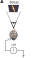
\includegraphics{media/chapters/02_modelling/02_02/visual_cortex_tuning_setup.pdf}%
	\includegraphics{media/chapters/02_modelling/02_02/visual_cortex_tuning.pdf}
	\caption[Neural tuning in the visual cortex]{Neural tuning in the visual cortex.
	\textbf{(A)} Illustration of the original experiment by \citet{hubel1959receptive}. Bright rectangles are briefly presented on a dark screen to an animal while recording from a neuron in its visual cortex. \textbf{(B)} Recorded spike trains for different stimulus orientations. Horizontal lines are the stimulus presentation interval. Adapted from \citet[Figure~3]{hubel1959receptive}. \textbf{(C)} The mapping between stimulus $\vec x$ and activity $a$ forms a \emph{tuning curve}. This neuron is tuned to vertical bars.}
	\label{fig:visual_cortex_tuning}
\end{figure}

%Given that we can simulate large biological systems at different levels of abstraction, the primary challenge is to construct networks that actually give rise to the behaviours observed in nature.
%Unfortunately, in many cases, too much about the brain is still unknown to successfully build such models.
%This is particularly true for brain regions involved in higher level cognition, and that, in terms of connectivity, are farther away from the periphery.
%Fortunately, brain regions \emph{closer} to the periphery are, relatively speaking, quite well understood.
%\footnote{Neuroscience textbooks such as \citet{kandel2012principles} discuss the neural circuitry of brain regions involved in sensory and motor processing in great detail, while chapters concerning higher-level cognitive tasks mostly report behavioural observations and coarse measurements such as fMRI scans.}
There are two important concepts that shed some light onto the organisation of brain networks---at least those brain networks involved in sensory processing: \emph{tuning curves} and \emph{receptive fields}.
In turn, these ideas motivate \emph{population codes}, which we heavily rely on in the context of our modelling tool, the Neural Engineering Framework---we discuss this in the next section.

\subsubsection{Tuning curves}
%Early studies on these concepts were conducted by \citeauthor{hubel1959receptive}.
In a famous \citeyear{hubel1959receptive} experiment (cf.~\Cref{fig:visual_cortex_tuning}), Hubel and Wiesel present a visual stimulus in the form of a bright rectangle at different orientations $\varphi$ to an experimental animal.
At the same time, the activity of a neuron in the animal's visual cortex is recorded.
This characterizes how the stimulus propagates through the brain up to the recording site.
%We characterize neurons in terms of their own physiological properties \emph{and} in terms of the preceding network connectivity.

In the recording depicted in \Cref{fig:visual_cortex_tuning}, we find that the neuron is most sensitive to---or, \emph{tuned} to---a certain orientation $\varphi$.
We could say that in this specific case, vertical bars are the \emph{preferred stimulus} of the neuron.
Generally, such a mapping from a stimulus property $\varphi$ onto the average neural activity $a(\varphi)$ is called a \emph{tuning curve} \citep[e.g.,][p.~1112]{vandenbos2015apa}\index{neuron!tuning curve}\index{tuning curve}.

\subsubsection{Receptive fields}

\begin{figure}
	\centering
	\includegraphics{media/chapters/02_modelling/02_02/gabor_filters.pdf}
	\caption[Examples of randomly generated of Gabor filters]{Examples of randomly generated Gabor filters.
	Each filter is a two-dimensional function $e(\xi_1, \xi_2)$, where $(\xi_1, \xi_2)$ is a spatial location.
	Negative  values (red) indicate that neural activity is reduced if a stimulus is present at that location, positive values (blue) indicate an increase in activity.}
	\label{fig:gabor}
\end{figure}
The concept of \emph{receptive fields}\index{neuron!receptive field}\index{receptive field} is closely related to tuning curves.
This is best illustrated in the context of stimuli that can be described as an intensity over a two-dimensional surface---such as vision or touch.
Generally, the receptive field of a neuron is the collection of points $(\xi_1, \xi_2)$ at which the presence of a stimulus---a point of light or mechanical pressure---triggers a neural response.
However, as evidenced by \citet{hubel1962receptive}, neural receptive fields are not only characterised in terms of the locations where a stimulus \emph{increases} the average neural activity, but also where the presence of a stimulus \emph{decreases} activity.

Mathematically, we can describe this in terms of a function $e(\xi_1, \xi_2)$ that assigns a weight to each stimulus location $(\xi_1, \xi_2)$.
This function $e$ is the receptive field.
\emph{Gabor filters}\index{Gabor filter} are a class of mathematical functions that fit observed receptive fields in the visual cortex well \citep{marcelja1980mathematical,field1986structure}.%
\footnote{Gabor filters are sinusoidals scaled by a radial Gaussian envelope. Such functions are maximally localised in time and space, as pointed out in the context of Gabor's Fourier uncertainty principle \citep{gabor1946theory}.}
Examples are depicted in \Cref{fig:gabor}.

Borrowing some notation from the next section, the activity of the neuron $a(x)$ can be modelled as the product between the receptive field $e$ and the stimulus $x$ integrated over space (where $x(\xi_1, \xi_2)$ is a function describing the stimulus intensity at a certain location)
\begin{align}
	a(x) &= G\left[ \alpha \iint e(\xi_1, \xi_2) x(\xi_1, \xi_2) \,\mathrm{d}\xi_1\mathrm{d}\xi_2 + \beta \right]
		= G \bigl[ \alpha \langle e, x \rangle + \beta \bigr] \,.
	\label{eqn:tuning_curve_from_receptive_field}
\end{align}
Here, $\langle e, x \rangle$ is the inner product between the receptive field and the stimulus (see \Cref{app:functional_analysis} for an introduction to functional analysis and the corresponding definitions).
Furthermore, $G$ is a rate approximation of the neuron model (see previous subsection), and, $\alpha > 0$ and $\beta$ translate the inner product into a neural input current.

Importantly, if the stimulus and receptive field are normalised, then $\langle e, x \rangle$ is the cosine similarity between the two functions.
Correspondingly, according to the above model, the neural response is maximised if $e = x$.
In other words, the receptive field \emph{is} the \enquote{true} preferred stimulus of a neuron.
This is consistent with modern definitions of the term \enquote{receptive field} in the neuroscience literature \citep[cf.][]{troy2009retinal}.

\begin{figure}
	\centering
	\includegraphics{media/chapters/02_modelling/02_02/visual_cortex_receptive_field_example.pdf}
	\caption[Model of the Hubel and Wiesel experiment]{Model of the original Hubel and Wiesel experiment (cf.~\Cref{fig:visual_cortex_tuning}). \textbf{(A)} The receptive field $e(\xi_1, \xi_2)$ describes whether a stimulus location $(\xi_1, \xi_2)$ acts excitatory (blue), or inhibitory (red). \textbf{(B)} The stimulus is a light rectangle at different orientations $\varphi$; this can be described as a function $x$ mapping locations onto light intensity. \textbf{(C)} Tuning curve obtained according to the model in \cref{eqn:tuning_curve_from_receptive_field}.}
	\label{fig:visual_cortex_receptive_field_example}
\end{figure}

\Cref{fig:visual_cortex_receptive_field_example} illustrates the relationship between the receptive field of a neuron and one of its tuning curves.
Choosing a vertically oriented Gabor filter as a receptive field, we can model the orientation tuning from the original Hubel and Wiesel experiment.
Thus, in a nutshell, a tuning curve is a characterisation of the neuron in terms of a specific stimulus property (e.g., the orientation of a bar of light), whereas the receptive field models its tuning properties in general (e.g., the predicted activity for any visual stimulus).

\subsubsection{Population codes}
Although tuning curves and receptive fields are inherently reconstructed from a network context, they still only characterise individual neurons.
To better understand biological neural networks, we need to consider the tuning properties of groups of neurons.

Doing this, we find that neighbouring neurons often have similar tuning properties---they are tuned to the same sensory modality, and possess similar receptive fields \citep{berkowitz2009population}.
Again, this has been explored well in context of orientation tuning in the visual cortex \citep[Chapter~25]{kandel2012principles}.
For example, neurons in visual cortex are organised in \enquote{cortical columns}.
Each column consists of several layers of neurons.
Within a single layer of the same column, neurons possess the similar preferred orientations.
Between columns, preferred orientations differ significantly.

This, as well as several other observations \citep{yuste2015neuron}, suggest that brain networks use \emph{population codes}.
The idea is that a single underlying quantity---such as the orientation of a visual stimulus---is represented by a group of neurons in a distributed manner.
The opposite would be \enquote{single-neuron coding}, where the activity of individual, localised neurons maps onto some quantity, or, in higher-level cognition, onto specific concepts \citep{berkowitz2009population}.

\begin{figure}
	\centering
	\includegraphics{media/chapters/02_modelling/02_02/population_code.pdf}
	\caption[Probabilistic decoding of scalar quantities using population codes]{Probabilistic decoding of scalar quantities using population codes.
	\textbf{(A)} \emph{Left:} The activity $a$ of a single neuron represents a scalar value $x \in [-1, 1]$.
	The current $J$ fed into each neuron is subject to Gaussian noise with standard deviation $\sigma = \SI{1}{\nano\ampere}$.
	Solid line corresponds to the median activity for the given represented value; shaded area corresponds to a contour line of the underlying probability density.
	\emph{Right:} Trying to decode the represented value $x$ from the activity results in significant uncertainties; negative values cannot be disambiguated. Dotted line is the optimum; solid line the median of a maximum-likelihood estimate, shaded area a contour line of the underlying probability density.
	Error $E$ is the decoding RMSE.
	\textbf{(B, C, D)} The larger the number of neurons, the smaller the uncertainties.}
	\label{fig:population_code}
\end{figure}

Population codes are intriguing as a model for representation in biological networks.
They allow precise inferences from imprecise or ambiguous observations. This is illustrated in \Cref{fig:population_code}.
For example, we can imagine that a single neuron represents a scalar value $x \in [-1, 1]$ as expressed by its tuning curve $a(x)$.
Unfortunately, the firing rate $a$ cannot be measured without error.
That is, neurons produce spontaneous activity that, as far as we can tell, is not related to a stimulus.
This is part due to noise inherent to neurobiological processes \citep[cf.][Section~2.2.1]{eliasmith2003neural}, and in part due to the Fourier uncertainty principle\index{Fourier!uncertainty principle}.%
\footnote{We can either estimate the frequency (i.e., rate) of a signal with a high precision at a low temporal resolution, or estimate the frequency with a low precision at a high temporal resolution \citep{gabor1946theory}.}
Hence, when trying to \emph{decode} the represented value $x$ from the neural activity, there is a large degree of uncertainty.
Adding neurons that are tuned to the same quantity $x$, but with different tuning curves to the population drastically reduces this uncertainty from a information-theoretic perspective \citep{ma2009population}.
